% !TEX root = thesis.tex
\documentclass[thesis.tex]{subfiles} 
\begin{document}

\chapter{Implementation}
\label{chap:impl}

In this chapter we will walk through the implementation of the pre-parsing tool
and the client library. We begin by detailing the process of parsing
mustache templates.

\section{Parsing mustache templates}
Our language of choice for implementing the parser is Haskell.
We utilize the Parsec parser combinator library to analyze our mustache
templates. With Parsec we can convert an EBNF grammar very effortlessly
into Haskell code by using the combinators and parsers the library supplies
us with.

\subsection{Mustache EBNF}
The EBNF for mustache is fairly simple and can be seen in figure
\ref{fig:mustache.ebnf}.
The behavior of the \inline{set\_delimiter} tag is ignored in this EBNF.

\begin{figure}
	\centering
	\setlength{\grammarindent}{3.5cm}
	\begin{grammar}
<variable> ::= `{{{' <ident> `}}}' | `{{&' <ident> `}}' | `{{' <ident> `}}'

<section> ::= `{{#' <ident> `}}' <content>* `{{/' <ident> `}}'
         \alt `{{^' <ident> `}}' <content>* `{{/' <ident> `}}'

<partial> ::= `{{>' <ident> `}}'

<comment> ::= `{{!' <comment> `}}'

<set\_delimiter> ::= `{{=' <delim\_start>  ' ' <delim\_end> `=}}'

<tag\_or\_char> ::= <section>
               \alt <partial>
               \alt <comment>
               \alt <set\_delimiter>
               \alt <variable>
               \alt <char>

<content> ::= <tag\_or\_char>*
	\end{grammar}
	\caption{Mustache EBNF}
	\label{fig:mustache.ebnf}
\end{figure}

\subsection{Mustache-XML EBNF}
\label{sec:mustache-xml-ebnf}
We want our parser to not only be able to understand mustache, but also HTML
intermingled with it. As such we extend our mustache grammar to incorporate
HTML as well.

There are many flavors of HTML we may choose from to allow in our
combined mustache-HTML grammar. To simplify our approach we will only allow well
structured XML tags, as this should ostensibly cover most of HTML.
HTML 5 allows for self-closing tags on void elements, which with our choice is
not something we can support. We will therefore refer to HTML tags in our
templates as XML tags.
\todo{Clarify that this does not mean we will cover XML with namespaces and all that jazz}

We build an abstract syntax tree with Parsec, in order for our tool to be
able to create DOM paths through this tree.
The EBNF in figure \ref{fig:mustache-xml.ebnf} represents the structure our
parser understands.

\begin{figure}
	\centering
	\setlength{\grammarindent}{4.2cm}
	\begin{grammar}
<variable> ::= `{{{' <ident> `}}}' | `{{&' <ident> `}}' | `{{' <ident> `}}'

<partial> ::= `{{>' <ident> `}}'

<content\_section> ::= `{{#' <ident> `}}' <template\_content>* `{{/' <ident> `}}'
                  \alt `{{^' <ident> `}}' <template\_content>* `{{/' <ident> `}}'

<attribute\_section> ::= `{{#' <ident> `}}' <attribute\_content>* `{{/' <ident> `}}'
                    \alt `{{^' <ident> `}}' <attribute\_content>* `{{/' <ident> `}}'

<comment\_section> ::= `{{\#' <ident> `}}' <comment\_content>* `{{/' <ident> `}}'
                  \alt `{{^' <ident> `}}' <comment\_content>* `{{/' <ident> `}}'

<content\_mustache\_tag> ::= <content\_section> | <partial> | <comment> | <variable>

<attribute\_mustache\_tag> ::= <attribute\_section> | <partial> | <comment> | <variable>

<comment\_mustache\_tag> ::= <comment\_section> | <partial> | <comment> | <variable>

<attribute> ::= ` ' <ident> `=\"' <attribute\_content>* `\"' 

<xml\_tag> ::= `<' <ident> <attribute>* `>' <template\_content>* `</' <ident> `>'
          \alt `<' <ident> <attribute>* `/>'
          \alt `<!--' <comment\_content>* `-->'

<attribute\_content> ::= <attribute\_mustache\_tag> | <char\_without\_doublequote>

<comment\_content> ::= <comment\_mustache\_tag> | <char>

<template\_content> ::= <content\_mustache\_tag> | <xml\_tag> | <char>

<content> ::= <template\_content>*
	\end{grammar}
	\caption{Mustache-XML EBNF}
	\label{fig:mustache-xml.ebnf}
\end{figure}

The mustache comment tag has been left out in this grammar, since it does not
output any content our client library can retrieve. We did also not include the
\inline{set\_delimiter} tag. This was mostly done to keep our first
implementation of the tool simple.

Using this grammar we can construct an abstract syntax tree
(figure \ref{fig:ast.ast}) from the mustache template in figure
\ref{fig:ast.mustache}.

\begin{figure}
	\centering
	\begin{subfigure}{\linewidth}
		\caption{A mustache template}
		\label{fig:ast.mustache}
		\begin{lstlisting}[language=JSON]
<div>
	Hello {{#user}}<a href="/user/{{id}}">{{name}}</a>{{/user}}
	<img src="about:blank" />
</div>
		\end{lstlisting}
	\end{subfigure}
	
	\begin{subfigure}{\linewidth}
		\caption{Abstract syntax tree generated by figure \ref{fig:ast.mustache}}
		\label{fig:ast.ast}
		\resizebox{\linewidth}{!}{% !TEX root = ../thesis.tex
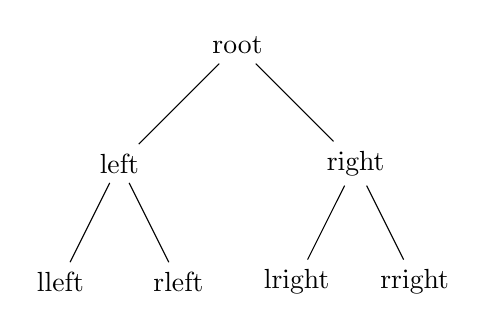
\begin{tikzpicture}[level distance=1.5cm,
  level 1/.style={sibling distance=3cm},
  level 2/.style={sibling distance=1.5cm}]
  \node {root}
    child {node {left}
      child {node {lleft}}
      child {node {rleft}}
    }
    child {node {right}
    child {node {lright}}
      child {node {rright}}
    };
\end{tikzpicture}
}
	\end{subfigure}
	\caption{Converting a mustache template to an abstract syntax tree}
	\label{fig:ast}
\end{figure}

\subsubsection{XML Comments}
An XML comment is recognized as simple text in the DOM of the browser. The EBNF
still allows for mustache tag structures. This allows the user to communicate
additional information to the client, without showing it in the browser.

\subsubsection{Template constraints}
\label{sec:template-constraints}
Note that the EBNF restricts the types of
templates our tool can parse.

\begin{itemize}
\item XML tags must be closed in the same template and section as they are opened.
\item Sections must adhere to the same structure as XML tags\footnote{
      This also means that sections may not interleave, something mustache
      does not support in any case}.
\item Variables and section may not exist in the identifier part of an XML tag
      or attribute.
\end{itemize}

A user may not run into these structural restrictions very often. Regardless,
they give our client library very useful guarantees about the rendered templates
it parses. They also allow us to create proper abstract syntax trees for any
template.
If XML tags were to be opened outside the scope of a template
and closed in the template we are parsing, there would be no way to determine
the location of mustache tags in the DOM without performing complicated
cross-references with the template that opened these tags.

\subsubsection{Character References}
The EBNF omits character references (e.g. \inline{\&nbsp;}, \inline{\&aring;}).
When those character references are accessed via the DOM in the browser they are
returned in their interpreted form. This forces our tool to also be able to
understand character references. To that end we simply scan any text we have
recognized between tags for ampersands, all characters from that point on until
a semicolon is found are passed to the \inline{lookupEntity} function available
in the TagSoup library (\todo{Ref to Text.HTML.TagSoup.Entity}), which converts
XML character references to UTF-8 characters.

\subsubsection{Lexeme token parsers}
Parsec can create token parsers given a configuration with definitions of
allowed operator letters, reserved operator names,
legal identifier letters and many other pieces of information
that are useful for parsing tokens in a language.
The token parsers returned by Parsec are lexeme token parsers.
These token parsers consume any whitespace that follow most tokens.
They also throw errors when tokens are followed by operator letters.

\subsubsection{Significant white spaces}
In the case of our template parser, the otherwise advantageous properties
of lexeme token parsers are not desirable.
White spaces in the beginning of an attribute value or after an XML tag can be
very significant.
We will need to be sure when a mustache variable begins and ends.
If a variable is surrounded only by white spaces, our tool will convey
data to the client which details that there is in fact no white space.
Subsequently the client will assume the white spaces recognized in the
rendered template belong to the value of the variable.

\subsection{Alternative parsing strategies}
Instead of Parsec we could have chosen an existing parsing technology for XML
and simply extended it.

\subsubsection{HXT (Text.XML.HXT)}
Haskell XML Tools (HXT) is a very advanced XML parser utilizing, amongst other
Haskell concepts, arrows. It is intended for querying structures the
tool creates by parsing the XML. Using it to discover the structure
of documents is not its main purpose. With this tool, we would have to create a
new structure on top of the existing HXT XML structure.

\subsubsection{XML (Text.XML.Light)}
XML is an easy-to-use XML library, which exports its data constructors.
This allows our functions to pattern match the data records the library has
created.
Mustache tags have to be recognized by inspecting all strings in the
structure we receive. After recognizing the tags, we have to overlay the
existing XML structure with section beginnings and ends and variable and partial
locations.
These overlay techniques would quickly outnumber the 250 lines of code our
Parsec parser spans now.

\section{Mustache-XML DOM Paths}
\label{sec:paths}
The abstract syntax tree our parser generates bears some resemblance to the
Document Object Model available in the browser. There is however the addition of
mustache section nodes and mustache variable/partial leafs.
Once the template is rendered, a mustache section will not be visible and the
contents of that section will be joined with the siblings of said section.
Similarly, mustache variables output text which will be joined with neighboring
text nodes. When constructing DOM paths this fact has to be taken into account.

\subsection{Resolver}
\label{sec:resolver}
Our tool passes the abstract syntax tree generate by the parser into a resolver.
The resolver links mustache tags together and analyzes dependencies between
them by creating ``Resolutions''. These resolutions have fields to point at
parent sections and neighboring nodes. They are used to access relevant parts of
our custom DOM more quickly.

\subsection{Lists of numbers as paths}
There are several ways to pinpoint a node in the DOM. CSS-selectors, XPaths and
DOM API-call chains among them. The first two methods are easily
readable and writable for humans, a feature we are not interested in.
Our tool is only intended to output information our client library can read.
We will instead use the third option: DOM API-call chains. However cumbersome
and counter-intuitive a method like this may seem in other scenarios, it is
in fact the optimal tool for our purposes: We are never interested in retrieving
more than a single DOM node; knowing where a section or a variable begins is our
only goal for paths.

All children of a node are ordered and can be addressed by numbers. This allows
us to drill down through the DOM to a specific node by iterating through a list
of numbers, descending one node generation with each iteration.

\subsubsection{Children and offsets}
\label{sec:children-offsets}
Paths for our mustache tags can be divided into two types which we will call
children and offsets.

Offsets are mustache tags whose location is affected by the string length of a
previous variable value or by the amount of iterations of a previous section.
To determine their location we will have to know the value of these previous
tags first. The tags may of course also only be offsets, therefore this chain
continues until we meet a parent section or the beginning of the template.

Children are tags with locations in the template that are not affected by
the value of a previous tag.
When parsing a rendered template in the client library, we will want to parse
all children first and continue with offsets that depend on those children.

Figure \ref{fig:section-example.mustache} from chapter \ref{chap:tools}
illustrates the difference very well, once we add a last list element as
shown in figure \ref{fig:offsets.mustache}.
\begin{figure}
	\centering
	\begin{lstlisting}[language=HTML]
	<p>
		Hello {{nickname}},<br/>
		you have {{messagecount}} new messages:
	</p>
	<ul>
		{{#messages}}
		<li>{{subject}} from {{nickname}}</li>
		{{/messages}}
		<li>That's all {{realname}}</li>
	</ul>
	\end{lstlisting}
	\caption{Offsets in templates}
	\label{fig:offsets.mustache}
\end{figure}
The \inline{\{\{realname\}\}} variable can only be retrieved once we know how
many times the messages section has iterated (in this case we could also look
for the last \inline{<li>} element, this is however not an approach that is
easily generalized). The path for \inline{\{\{realname\}\}} would consist of
two numbers as highlighted in figure \ref{fig:messages.ast}.
\begin{itemize}
\item The node index of the \inline{<li>} element measured from
      the closing tag of the \inline{\{\{\#messages\}\}} section.
      Also counting the text node between those tags, we arrive at \emph{1}.
\item The node index of the \inline{\{\{realname\}\}} variable. Although this
      variable will be merged with the previous text, our tool still counts it
      as a separate node. We will adjust for this way of counting child nodes in
      the client library. Here we also arrive at index \emph{1}.
\end{itemize}

\begin{figure}
	\centering
	\resizebox{\linewidth}{!}{% !TEX root = ../thesis.tex
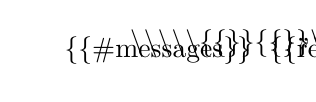
\begin{tikzpicture}
\tikzset{level distance=60pt,sibling distance=5pt}
% <ul>
% 	{{#messages}}
% 	<li>{{subject}} from {{nickname}}</li>
% 	{{/messages}}
% 	<li>That's all {{realname}}</li>
% </ul>
\Tree [.{<ul>}
	{"\textbackslash n\textbackslash t"}
	[.\node(msg){\{\{\#messages\}\}};
		{"\textbackslash n\textbackslash t\textbackslash t"}
		[.{<li>}
			{\{\{subject\}\}}
			{" from "}
			{\{\{nickname\}\}}
		]
		{"\textbackslash n\textbackslash t\textbackslash t"}
	]
	\node(txt){"\textbackslash n\textbackslash t\textbackslash t"};
	[.\node(li){<li>};
		{"Thats all "}
		\node(realname){\{\{realname\}\}};
	]
	{"\textbackslash n\textbackslash t"}
]
\draw[dashed,->] (msg)--(txt);
\draw[dashed,->] (txt)--(li);
\draw[dashed,->] (li)..controls +(east:2) and +(east:2)..(realname);
\end{tikzpicture}
}
	\caption{The path from \inline{\{\{\#messages\}\}} to \inline{\{\{realname\}\}}}
	\label{fig:messages.ast}
\end{figure}

The only detail missing from our new path is the reference to the node we are
offsetting from. By assigning a number to each mustache tag in the template we
can refer to it by that number and prepend it to our path.

Child paths are generated in much the same way. We proceed in the exact same way
as with the \inline{\{\{realname\}\}} variable, if we were to generate a path
for the \inline{\{\{subject\}\}} variable in template \ref{fig:offsets.mustache}.
The only difference lies in the classification of the path as a child instead of
an offset.
The advantage we gain by this classification is our ability to distinguish
whether a variable is located inside or outside the section.

\section{Variable boundaries}
Variables embedded in text nodes will be merged with the neighboring text nodes
once a template is rendered. To extract the original text, the client library
will have to know the exact length of the text before and after it. If two
variables are located in the same text node, this extraction strategy is no
longer possible. Instead we simply remember the text surrounding the variable.
Using this prefix text our client library can not only find the beginning of a
variable, but also verify the preceding text. The succeeding text will be
used as a delimiter, it marks the end of our variable.
With this strategy we can parse an arbitrary number of variables in one text
node, provided a variable does not contain the text of the succeeding
text\footnote{Why we cannot parse in a different way is detailed in
\ref{sec:var-boundary-ambiguity}}.

\subsection{Other boundaries}
The previous and next nodes of a variable may also be HTML or mustache tags.
In the case of an HTML tag, we will simply relay the name of the tag to the
client library. If the variable is the first or last node, the client library
will receive a special ``null node'' as the previous or next node respectively.
We will tackle the case of neighboring nodes being mustache tags in
\ref{sec:lookahead}.

\section{Recognizing iterations}
To detect whether a section is skipped because its value is an empty
list or false, we let the client library know what the first child of the
section is.
This way we can detect if a section in a rendered template begins with the
first child node and has content or begins with its neighboring next node and is
empty.

\subsection{Content list}
\label{sec:content-list}
We accompany each section with a list of child node types. The client library
shall consult this list to determine the length of each iteration.
The length of an iteration is constant if a section only contains normal
HTML tags as its children. Once we introduce mustache tags as children\footnote{
	Note the important distinction of ``children'' and ``descendants''.
	A section may contain an XML node with mustache tags inside it.
	Those do however not affect the \inline{childNodes} list of the parent tag.
} of the
section, this changes.
The length of a subsection will increase the length of a parent section, while
unescaped variables may do the same.
In order for us to still reliably determine said length, we also include
mustache tags in this content list. The client library may then access
information about these tags to asses the impact they have had on the length of
an iteration.
\todo{Eval: this can be done a lot easier}

\subsection{Lambda sections}
Lambda sections and normal mustache sections can not be distinguished.
We also have no way of determining the input to a function by looking at its
output. For that reason we will simply treat them as sections when parsing
templates and assume the user is aware when a function is bound to a dataset
instead of any type of value.

\subsection{If-else constructs}
\label{sec:if-else}
Sections which are intended as if-else constructs are similarly impossible to
distinguish from normal sections, which iterate over a list. We tackle this
issue by regarding all sections as iterative sections. We return a list of
entries, regardless of the original dataset structure that was fed in to the
template rendering engine.
This behavior is also in accordance with the mustache spec:
\begin{citequote}{\cite[sections.yml]{MSTSPEC}}
	if the data is truthy (e.g. `!!data == true`), use a single-element list
	containing the data, otherwise use an empty list.
\end{citequote}

\section{Outputting information}
\label{sec:output}
We transmit the information our tool retrieves from templates to the client
library using the JSON data format. Our tool generates the output by using the
JSON library available in the ``Hackage'' Haskell library database (Text.JSON).

JSON files may contain an array or an object as the top-level structure.
We choose to use an array, in which each entry describes a mustache tag.
Referencing between those tags functions by way of the index\footnote{
	This index is the same number we prepend to the paths of tags in section
	\ref{sec:children-offsets}
} in said array.
We also prepend a ``root'' section to the array. It is referred to by mustache
tags that are not located inside a section and are not offset in their location
by other mustache tags.


\todo{Difference between parser combinators and parser generators}
\todo{What about cabal, cmdargs?}

\section{Client library}

\subsection{Technology choices}

\subsubsection{CoffeeScript}
We use CoffeeScript to program our client library. The language allows us to 
write expressions very tersely, where plain JavaScript would have required
verbose instructions. This helps us to overview more code at once.
CoffeeScript constructs like \inline{unless exp}, which translates to
\inline{if(!exp)}, also help highlight the control flow in a semantically
better way.

\subsection{Input}
The client library expects the user to hand it both the rendered template and
the template information our pre-parser tool outputs.
How this data is retrieved is not the concern of the library.
The rendered template is expected to already be in the DOM format.
Additionally it needs to be wrapped in a container node,
which is the actual node that is to be handed to the library.
The client library also expects the JSON data to already have been interpreted
and converted to JavaScript objects.

\subsection{Representing mustache tags}
Our architecture for representing mustache tags is a one-to-one representation
of the possibilities in mustache.
Each section object holds all of its iterations. A section, variable or partial
in a section is instantiated as many times as the section iterates.

\subsubsection{Offsets}
Through the whole process, we will maintain two pointers that identify our
progress in the rendered template:
\begin{itemize}
\item \inline{nodeOffset}: Given a parent, this variable indicates the index
      in the \inline{childNodes} list we are currently pointing at (node offset).
\item \inline{strOffset}: Assuming the current node is a text node, this variable
      points at the current string position (string offset).
\end{itemize}

For all mustache tags, we will always keep a reference to the \inline{parent}
XML node it is located in. This allows us to increase and decrease the
\inline{nodeOffset} to access neighboring nodes. This would also be possible by
using the \inline{previousSibling} and \inline{nextSibling} properties,
mathematical operations like ``the 5th neighbor of the current node'' will
however become quite intricate.

The node offset and string offset is maintained separately for each mustache tag
object. An object is instantiated with those offsets, giving it a position to
follow its path from and find its node.

\subsubsection{Following DOM paths}
Given the position (\inline{nodeOffset}, \inline{strOffset} and \inline{parent})
of a mustache tag, we locate other mustache tags that have their location
specified relative to it by executing the following steps for each entry in
their respective path array
excluding the first entry, which is a mustache tag reference
(see \ref{sec:children-offsets}):
\begin{itemize}
\item Add the current entry to the \inline{nodeOffset}
\item Break, if this is the last entry
\item Set the parent node to point at the childNode index \inline{nodeOffset} of
      the current parent node
\end{itemize}
We break in step 2 to let the parent point at the parent of the mustache tag
instead of the tag it has been replaced with.

If an entry in the iteration is a string instead of an integer, this indicates
an attribute name. In that case we set the parent node to be the attribute node
the string identifies.
Attribute nodes support the childNodes property in the same way an element node
does.

The string offset is reset to 0 once we leave the string context of the
current text node. This happens when there is an XML tag between the
mustache tag the path is based on and the node the path points at.

\subsection{Parsing sections}
The parsing of sections constitutes the heart of operations in our library.
We bootstrap our parser by initializing the fake root section
(see \ref{sec:output}) with the template container node as its parent.
The root section will of course only have one iteration.
This method allows us to create a recursive parsing process which we will
initiate once per iteration for each section we encounter inside a section.

Inside an iteration we will also instantiate variables and partials that are
children of the current section. Any mustache tag located inside a subsection
will be handled by that section.

We begin by instantiating all mustache tags that are not offsets. These
tags have their location described relative to our section, of which we know the
location. This means that we can determine their location without any other
dependencies.
Note that we in each section iteration adjust the node offset
to point at the node before the first node in the current iteration.
This ensures that the path following process works correctly.

Next we instantiate all tags that are offset by a preceding mustache tag.
Since our tool outputs information about tags in the order they appear in, in the
template, we simply iterate through the mustache tags, knowing we will not
encounter a tag with an offset pointing at a yet uninstantiated node.

Once all tags in a section are instantiated and saved in an object mapped by
their identifier, we determine the length of our section with the content list
as described in section \ref{sec:content-list}. This length is used to adjust
the section node offset. Using it, mustache tags basing their path on this
section can locate their node.

Depending on whether the node following the current node can be identified as
a first child of the section or as a neighboring node, we either begin another
iteration or terminate the parsing process for this section.

\subsubsection{Parsing partials}
\label{sec:parsing-partials}
Partials can be handled by simulating the beginning of an entirely new template.
Provided the partial is enclosed in an XML tag, we can
restart the parsing process using the matching template information for that
partial.

\subsection{Joined text nodes}
\label{sec:joined}
Our pre-parser tool recognizes a section with preceding text and text inside it
as two nodes with the section containing a third node. In a rendered template
these three nodes will merge into one single text node. Variables will also
merge with any preceding text node. Succeeding text has a similar effect.
This effect can wreak havoc on our node offsets if we do not adjust for it.
Sections will therefore detect whether their previous node is joined with
their first child and reduce the node offset by one. This is also done for:
\begin{itemize}
\item Previous nodes and next nodes
\item Last child nodes and next nodes
\item Last child nodes and first child nodes
\end{itemize}
In each of these cases we adjust the node offset accordingly. We adjust
for previous and next nodes of variables in the same way.

Figure \ref{fig:relationships.ast} illustrates these relationships between elements
and sections.

Note also how the DOM of a rendered template in figure \ref{fig:rendered} is
different from our abstract syntax tree in figure \ref{fig:relationships.ast}.
Sections no longer exist and text nodes that were previously separated have now joined.
Variables have similarly joined with adjacent text nodes.

\begin{figure}
	\centering
	\begin{subfigure}{\linewidth}
		\caption{A mustache template}
		\label{fig:relationships.mustache}
		\begin{lstlisting}[language=mustache]
<div>
	Meet and greet:{{#user}} Hello {{name}}<br/>{{/user}}
	<img src="about:blank" />
</div>
		\end{lstlisting}
	\end{subfigure}
	
	\begin{subfigure}{\linewidth}
		\caption{The relationships of a section in an abstract syntax tree generated
		         by figure \ref{fig:relationships.mustache}}
		\label{fig:relationships.ast}
		\resizebox{\linewidth}{!}{% !TEX root = ../thesis.tex
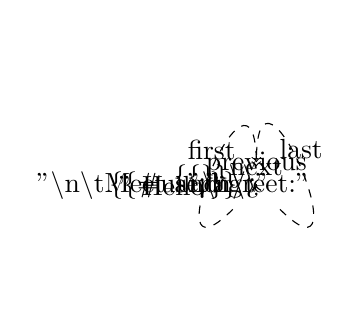
\begin{tikzpicture}
\tikzset{level distance=70pt,sibling distance=10pt}
%<div>
%	Meet and greet:{{#user}} Hello {{name}}<br/>{{/user}}
%	<img src="about:blank" />
%</div>
%
\Tree [.{<div>}
	\node(prev){"\textbackslash n\textbackslash tMeet and greet:"};
	[.\node(section){\{\{\#user\}\}};
		\node(first){" Hello "};
		{\{\{name\}\}}
		\node(last){<br/>};
	]
	\node(next){"\textbackslash n\textbackslash t"};
	[.{<img/>}
		{...}
	]
	{"\textbackslash n\textbackslash t"}
]
\draw[dashed,->] (section)--(prev) node [midway,above] {previous};
\draw[dashed,->] (section)--(next) node [midway,above] {next};
\draw[dashed,->] (section)..controls +(south west:2) and +(north:2)..(first) node [midway,left,above] {first};
\draw[dashed,->] (section)..controls +(south east:2) and +(north:2)..(last) node [midway,right,above] {last};

\end{tikzpicture}
}
	\end{subfigure}
	
	\begin{subfigure}{\linewidth}
		\caption{Input to the template in figure \ref{fig:relationships.mustache}}
		\label{fig:rendered.json}
		\begin{lstlisting}[language=JSON]
{ user: [ {name: "user1"}, {name: "user2"} ] }
		\end{lstlisting}
	\end{subfigure}
	
	\begin{subfigure}{\linewidth}
		\caption{Resulting HTML when rendering the dataset in \ref{fig:rendered.json}
		         using the template from figure \ref{fig:relationships.mustache}}
		\label{fig:rendered.html}
		\begin{lstlisting}[language=HTML]
<div>
	Meet and greet: Hello user1<br/> Hello user2<br/>
	<img src="about:blank" />
</div>
		\end{lstlisting}
	\end{subfigure}
	
	\begin{subfigure}{\linewidth}
		\caption{DOM tree for \ref{fig:rendered.html}}
		\label{fig:rendered.ast}
		\resizebox{\linewidth}{!}{% !TEX root = ../thesis.tex
\begin{tikzpicture}
\tikzset{level distance=70pt,sibling distance=10pt}
%<div>
%	Meet and greet: Hello user1<br/> Hello user2<br/>
%	<img src="about:blank" />
%</div>
%
\Tree [.{<div>}
	{"\textbackslash n\textbackslash tMeet and greet: Hello user1"}
	{<br/>}
	{" Hello user2"}
	{<br/>}
	{"\textbackslash n\textbackslash t"}
	[.{<img/>}
		{...}
	]
	{"\textbackslash n\textbackslash t"}
]
\end{tikzpicture}
}
	\end{subfigure}
	\caption{Tree transformations when rendering a mustache template}
	\label{fig:rendered}
\end{figure}

\subsection{Verifying nodes}
Previous nodes, next nodes, first children and last children are matched with
a single data structure.
They are specified with their type and in some cases, depending on the type,
a second parameter:
\begin{itemize}
\item \emph{emptynode}: A self-closing XML tag. The second parameter specifies
                        the tag name
\item \emph{node}:      An XML tag. The second parameter specifies
                        the tag name
\item \emph{comment}:   An XML comment. It has no second parameter.
\item \emph{text}:      A text node. The second parameter is the text itself.
\item \emph{null}:      No node (e.g. the variable is the
                        last child of an XML tag). The type has no second
                        parameter.
\end{itemize}

Conflicts may arise if e.g. the next node of a section and its first child are
indistinguishable. These cases can be detected by our pre-parsing tool with a
filtering mechanism.

\subsubsection{Filter}
\label{sec:filter}
Before our pre-parsing tool outputs the template information, it runs the
resolutions generated by the Resolver\footnote{See \ref{sec:resolver}}
through a set of filters.

\begin{itemize}
\item \emph{unescaped\_offset} Check if a any mustache tags use an unescaped
                               variable as their path base\footnote{
                               	Because of the \emph{unescaped\_pos} filter,
                               	this filter is actually superfluous.
                               }. \todo{Remove this filter from the code}
\item \emph{empty\_section} Check for empty sections. They should be removed.
\item \emph{unescaped\_pos} An unescaped variable may only be the last child
                            of an XML tag. It may not be a child of a section
                            (see \ref{sec:unescaped-variable-filter}).
\item \emph{partial\_only\_child} A partial must be the only child of an XML tag
                                  (see \ref{sec:partial-only-child}).
\item \emph{no\_lookahead} Neighboring nodes and first and last children may not
                           be mustache tags (see \ref{sec:lookahead}).
\item \emph{ambiguous\_boundaries} The first child of a section must be
                                   distinguishable from the next node of a
                                   section.
\item \emph{path\_with\_errors} Paths may not be based on tags that have
                                produced any errors.
\end{itemize}

We output a message if any of the filters fail and exclude that tag from the
output.

Having created all the phases necessary for our pre-parser tool to output the
right information, we can now overview the architecture in figure \ref{fig:tool-arch}.
\todo{explain the image}

\begin{figure}
	\centering
	\resizebox{\linewidth}{!}{% !TEX root = ../thesis.tex
\begin{tikzpicture}[every edge/.style={link}]
	\node[entity] (json) {JSON};
  \node[relationship] (generator) [left=of json] {Generator} edge [->] (json);
	\node[entity] (filtered) [left=of generator] {Resolutions (filtered)} edge [->] (generator);
  \node[relationship] (filter) [above=of filtered] {Filter} edge [->] (filtered);
	\node[entity] (resolutions) [right=of filter] {Resolutions} edge [->] (filter);
  \node[relationship] (resolver) [right=of resolutions] {Resolver} edge [->] (resolutions);
	\node[entity] (dom) [above=of resolver] {Mustache-XML DOM} edge [->] (resolver);
  \node[relationship] (parsec) [left=of dom] {Parsec} edge [->] (dom);
	\node[entity] (tpl) [left=of parsec] {Template} edge [->] (parsec);
	
  
  
	% \node[draw=black,thick,inner sep=2mm,rectangle,fit=(tplinfo) (tpl)] (static) {};
	% \node[anchor=north,inner sep=1mm] at (static.south) {Static content};
	
	% \node[draw=black,thick,inner sep=2mm,rectangle,fit=(mustache) (parser) (cdata)] (dynamic) {};
	% \node[anchor=north,inner sep=1mm] at (dynamic.south) {Dynamic content};
	
	% \begin{scope}[on background layer]
	% 	\node[fill=gray!20,inner sep=2mm,rectangle,fit=(mustache) (tpl) (tplinfo)] (server) {};
	% 	\node[anchor=south,inner sep=1mm] at (server.north) {Server};
		
	% 	\node[fill=gray!20,inner sep=2mm,rectangle,fit=(dom) (parser) (cdata)] (client) {};
	% 	\node[inner sep=1mm] at (client) {Client};
	% \end{scope}
\end{tikzpicture}
}
	\caption{Architectural diagram of the pre-parser tool}
	\label{fig:tool-arch}
\end{figure}

\subsection{Returning values}
We save all instantiated sections, variables and partials for every section
iteration. Once we have parsed a rendered template, we retrieve our root section
and generate a JavaScript array containing one anonymous object per iteration.
The object maps variable names to their parsed values and section names to their
iterations.
As noted in section \ref{sec:parsing-partials}, partials are considered
sections. Since partials in mustache behave as if the template was inlined,
we merge the contents of the partial section with the contents of the
parent section\footnote{
	As detailed in \ref{sec:parsing-partials} we handle partials like new
	templates, this means they only have one iteration like the root section.
}
Unescaped variables will return a list of their nodes as their value.
Previous and next nodes will be included if they are text nodes.

\subsubsection{Parent nodes}
\label{sec:parent-nodes}
We add a second useful value to the return value of variables. Often times a
user may want to listen to changes concerning the nodes in which mustache tags
are placed. Variables may be values in attributes on key XML tags
(e.g. value attributes in form input fields) in which case event listeners can
be added to those attributes and useful actions performed when they are
triggered.

\subsubsection{Update()}
\label{sec:update}
Variables also return an \inline{update(text)} function. Passing it a string
will update their substring in the text node and preserve the surrounding text.

\section{``Comb''}
The tool we have created will be named ``Comb''. It refers to the combing of
a mustache, much like we comb through templates and rendered templates to
retrieve mustache tags and variable values.

The template information generated by our pre-parser tool is called a
``comb file'', its file extension is ``.mustache-comb''.

\end{document}
